\section{Introduction}

\subsection{Topological data analysis}\label{sec-tda}
In this section, we will give an informal introduction to persistent homology, which we will make more rigorous in the following sections. In topological data analysis, we are interested in studying geometric datasets using the tools of algebraic topology. For example, let $X$ be the finite subset of $\R^2$ in Figure \ref{tda_1}. We consider this our dataset, and we want to detect that it has the shape of a circle.
\begin{figure}[h!]
    \centering
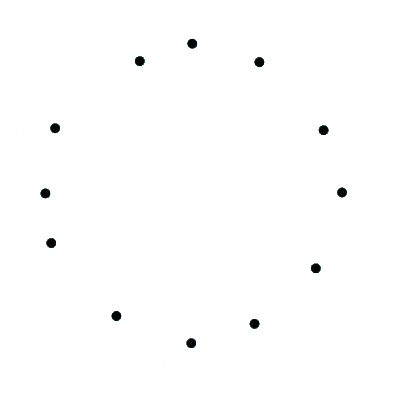
\includegraphics[width=0.3\textwidth]{tda_1.png}
    \caption{A geometric dataset in $\R^2$.}
    \label{tda_1}
\end{figure}
One idea is to, for each real $\epsilon \geq 0$, consider the subspace $X_\eps \subseteq \R^2$ given by the union of the closed balls of radius $\epsilon$ centered at each data point $x \in X$. For small $\epsilon$, this will be homotopy equivalent to the disjoint sum of various points, depending greatly on $\epsilon$ as points close to each other merge into one connected component. For large values of $\epsilon$, e.g larger than the radius of the perceived circle, $X_\eps$ is contractible. However, for Goldilock values of $\epsilon$, the space will be homotopy equivalent to $S^1$, as seen in Figure \ref{tda_2}. In fact, since $X$ is a finite set, there are only finitely many `interesting' values for $\eps$: those where two previously non-intersecting balls intersect.  We consider the $\R_\geq$-indexed sequence of spaces $X_\eps$ and their topological features as encoding the geometry of our original dataset.
\begin{figure}
    {\centering
    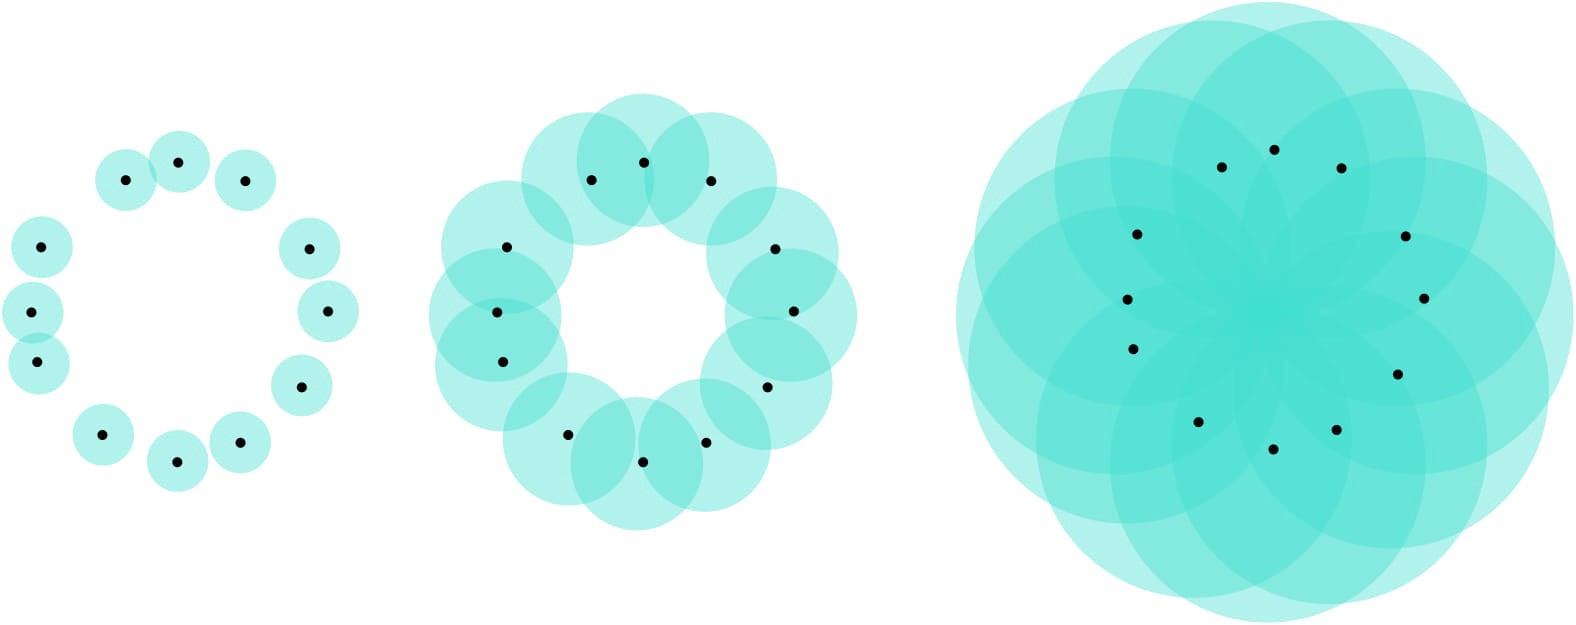
\includegraphics[width=\textwidth]{tda_2.jpeg}
    \caption{The subspace $X_\eps$ for three values of $\eps$.}}
    {\small Source: \url{https://towardsdatascience.com/a-concrete-application-of-topological-data-analysis-86b89aa27586}}
    \label{tda_2}
\end{figure}

We can detect the circle by taking singular homology with coefficients in some field $\F$ at each $\epsilon.$ This gives, for every nonnegative integer $n$ and every $\epsilon \geq 0$, a finite-dimensional $\F$-vector space $H_n(X_{\epsilon},\F)$, as well as maps $H_n(X_\epsilon,\F)\rightarrow H_n(X_{\eps'},\F)$ induced by the inclusion $X_\epsilon\xhookrightarrow{}X_\eps'$ whenever $\epsilon \leq \eps'$. As we will see in Section \ref{sec:barcodes}, we can always choose bases such that these maps send each basis element to either $0$ or another basis element. Moreover, we only need to consider finitely many values of $\epsilon$ where the space differs up to homotopy equivalence since $X$ is finite. We call these \textbf{critical values}. This allows us to represent the homology as a \textbf{barcode diagram}, as seen in Figure \ref{tda_3}. Each line represents a generator of $H_n(X_\epsilon,\F)$, and at each critical value, the line persists if the corresponding map in homology preserves that generator, and disappears if the corresponding map is $0$ on the generator. The diagram in Figure \ref{tda_3} is the $0$th homology barcode diagram, counting the number of path components. Short-lived bars are interpreted as noise, while long-living bars are interpreted as the true homology of our data set, informally called its persistent $0$\textsuperscript{th} homology. In this case, the persistent $0$\textsuperscript{th} homology tells us our data set has a single path component. If we define $H(X_\epsilon,\F)=\bigoplus_k H_k(X_\epsilon,\F)$ we can furthermore summarise all the homology groups in a single barcode diagram.
\begin{figure}[h!]
    \centering
    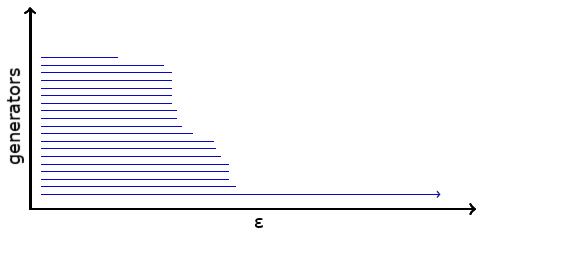
\includegraphics[width=0.8\textwidth]{tda_3.png}
    \caption{Barcode diagram in $0$th homology for the data set in Figure \ref{tda_1}.}
    \label{tda_3}
\end{figure}

\subsection{Interleaving distance}\label{sec-categorification}
We are interested in formalising persistent homology in the language of category theory, as this will allow us to compare persistent homology to other theories. We follow closely the approach in \cite{Bubenik2014}. 

In this section, $\Z$ and $\R$ will denote the poset category in the canonical way. We have an endofunctor $T_b:\R\rightarrow \R$ given by translation by $b$, as well as a natural transformation $\eta_b:id\rightarrow T_b$ whose components are given by $\eta_b(a):a\leq a+b$. This allows us to make the following definitions.

\begin{definition}[\cite{Bubenik2014}]\label{def:epsilon_interleaving}
Let $D$ be a category, and $F,G\in D^{\R}$ be $\R$-indexed diagrams in $D$. An $\epsilon$-interleaving $(F,G,\phi,\psi)$ of $F$ and $G$ consists of natural transformations $\phi:F\rightarrow GT_{\epsilon}$ and $\psi:G\rightarrow FT_\epsilon$ such that $(\psi T_\epsilon)\phi=F\eta_{2\epsilon}$ and $(\phi T_\epsilon)\psi=G\eta_{2\epsilon}$. If an $\epsilon$-interleaving exists, we say $F$ and $G$ are $\epsilon$-interleaved.
\end{definition}

%Let $D=\R$ and consider the diagrams $$F(\epsilon)=(-\epsilon,\epsilon) \text{ and }G(\epsilon)=(-\epsilon,\epsilon)\cup (1-\epsilon,1+\epsilon).$$


%Consider two finite data sets, seen as finite subsets of the metric space $A,B\subset\R^n$. In \ref{sec-tda}, we saw how this gives rise to $\R-$indexed diagrams valued in the category of finitely generated vector spaces $\textbf{Vec}$, namely $$F=H(A_{(-)},\F),G=H(B_{(-)},\F)$$ for some fixed field $\F$. If $F=G$ then trivially $F$ and $G$ are $\epsilon-$interleaved for any $\epsilon\geq 0$, by letting $\phi=\psi=G\eta_\epsilon$. (...)
    %If there is an interval $I$ with $|I|>\epsilon$ such that the barcodes of $F$ and $G$ differ on all of $I$, then $F$ and $G$ are not $\epsilon$-interleaved (PROVE). If all intervals where their barcodes differ are of length less than $\epsilon,$ then we can (...)

    %In other words, $F$ and $G$ are $\epsilon-$interleaved if the intervals where their barcode diagrams differ are less than $\epsilon$ in width.

\begin{definition}
    Given two $\R$-indexed diagrams $F,G$ in $D$ we define their \textbf{interleaving distance} as
    \[d(F,G)=\text{inf}\{\epsilon : \text{ $F$ and $G$ are $\epsilon$-interleaved}\}.\]
\end{definition}
For an example of the interleaving distance in action, see Example \ref{ex:interleaving-distance}. For now, we would like to show that $d$ is an \textbf{extended metric}, that is, one that can take the value $\infty$ (note $\text{inf}(\emptyset)=\infty.$) However, we do not a priori have that $d(F,G)=0\iff F=G$. To get around this, we define an equivalence class on $\R$-indexed functors, where $F\sim G\iff d(F,G)=0$. It is not difficult to see this is an equivalence relation. $F\sim F$ trivially, and $F\sim G\implies G\sim F$ by swapping $\phi$ and $\psi$ for each $\epsilon>0.$ Finally, $F\sim G, G\sim H\implies F\sim H$ by vertically composing the relevant $\phi$ and $\psi.$
\begin{lemma}
    The interleaving distance is an extended metric on the class of equivalence classes of $\R$-indexed functors in $D$ defined above.
\end{lemma}
\begin{proof}
Omitted. See \cite{Bubenik2014}.
\end{proof}

We are particularly interested in $\R$-indexed diagrams \textbf{Vec}, the category of finite-dimensional vector spaces. However, we will first take a small detour to prove a result about finitely generated $R-$modules.

\subsection{Structure Theorem for Graded PIDs} \label{sec:structurethm}

Recall the structure theorem for PIDs:

\begin{theorem} 
Let \(R\) be a Principal Ideal Domain. Suppose \(M\) is a finitely generated \(R\)-module, then \(M\) admits a decomposition
\[M \cong R^a \oplus \left(\bigoplus_{i=1}^{m}R/d_i R\right),\]
such that \(d_1|\cdots|d_m\). Moreover, the ideals $d_iR$ are uniquely determined; or, alternatively, the $d_i$ are uniquely determined up to multiplication by a unit.
\end{theorem}

In this section, we will prove a graded version of this, for \(M\) a graded module over \(R\) a graded PID.

\begin{theorem}\label{thm:GradedStructure}
Let \(R\) be a graded Principal Ideal Domain. Suppose \(M\) is a finitely generated graded \(R\)-module, then \(M\) admits a decomposition
\[M \cong \left(\bigoplus_{i=1}^{n}\Sigma^{\alpha_i} R \right)\oplus \left(\bigoplus_{j=1}^{m} \Sigma^{\beta_j}R/d_j R\right),\]
where \(\Sigma^{\alpha}\) refers to an upwards shift in grading by \(\alpha\), and the $d_j$ are homogeneous and uniquely determined up to multiplication by a unit.
\end{theorem}

The proof of this is very similar to the proof of the Structure Theorem of regular PIDs. We just need to be mindful when dealing with graded pieces\footnote{A full proof of this theorem could not be found in any literature we read, although it was alluded to in many papers.}. 

\begin{proof}
    Since \(M\) is finitely generated, let \(m_1,\dots,m_s\) be a set of homogenous generators of \(M\) with degrees \(\gamma_1,\dots,\gamma_s\). Then there exists a surjection of graded modules
    \[\phi:\bigoplus_{i=1}^{s}\Sigma^{\gamma_i} R \twoheadrightarrow M.\]
    Let \(S=\bigoplus_{i=1}^{s}\Sigma^{\gamma_i} R\). By the first isomorphism theorem, we know that \(M\cong S/\ker \phi\). Note that kernels of a graded morphism are also graded, so \(\ker\phi\) is a graded submodule of \(S\).

    By the Graded Smith Normal Form, there exists a suitable change of basis of \(\{m_i\}\) such that \(\ker\phi\) is generated by \(d_1m_1,d_2m_2,\dots, d_nm_n\) for some \(n\leq s\). Then the quotient is easily calculated to be
    \[M\cong S/\ker\phi \cong \frac{\displaystyle\bigoplus_{i=1}^{s}\Sigma^{\gamma_i} R}{\displaystyle\bigoplus_{i=1}^{n}d_i\Sigma^{\gamma_i} R} \cong \left(\bigoplus_{i=1}^{n}\Sigma^{\gamma_i} R/(d_i)\right) \oplus\left(\bigoplus_{i=n+1}^{s}\Sigma^{\gamma_i} R\right),\]
    which is precisely of the form stated in the theorem.
\end{proof}

The proof above assumes the existence of a Graded Smith Normal Form. We now provide an algorithm for finding the Smith Normal Form that respects grading. A statement of this algorithm the case of \(R=\F[t]\) can be found in \cite{Skraba2013PersistenceMA}.

\begin{lemma}[Graded Smith Normal Form]\label{thm:GradedSmith}
    Let $M=\bigoplus_{i=1}^{m} \Sigma^{\gamma_i} R$ with $\Sigma^{\gamma_i} R$ generated by $v_i$, and $N \leq M$ a graded submodule. Then there exist bases $\{v_1',\dots,v_m'\}$ and $\{w_1,\cdots, w_n\}$ for \(M\) and \(N\), respectively, such that \(n\leq m\) and \(w_i=d_iv_i'\) for some unique (up to multiplication to a unit) homogeneous \(d_i\in R\) satisfying \(d_1|\cdots |d_n\).
\end{lemma}

\begin{proof}[Proof sketch.]
    Suppose \(N\) is generated by some homogeneous \(x_1,\dots,x_n\), where \(x_j\) has degree \(\delta_j\). Without loss of generality, assume that the generators \(v_i\) and \(x_j\) are ordered in non-decreasing order of grading, i.e. \(\gamma_1\leq \gamma_2\leq \dots \leq \gamma_n\) and  \(\delta_1\leq \delta_2\leq \dots \leq \delta_n\). Since the \(v_i\) form a generating set, we can write \(x_j=\sum v_if_{ij}\) for some coefficients $f_{ij}$. In fact, we may take the $f_{ij}$ to be homogeneous, since any terms of degree different than $\delta_j$ must cancel. We can express this in terms of a matrix where each \(x_i\) is a column vector
    \[
    A =
    \begin{pmatrix}
        f_{11} & f_{12} & \cdots & f_{1n}\\
        \vdots & \vdots & \vdots & \vdots\\
        f_{m1} & f_{m2} & \cdots & f_{mn}
    \end{pmatrix}
    =
    \begin{pmatrix}
        \uparrow & \uparrow & & \uparrow\\
        x_1 & x_2 & \cdots & x_n\\
        \downarrow & \downarrow & & \downarrow
    \end{pmatrix}.
    \]
    Notice that by the homogeneity condition of the \(x_i\), the degrees of \(f_{ij}\) satisfy
    \[\gamma_i +\deg f_{ij}= \delta_j.\]

    In the standard proof of Smith Normal form, we can simply use row and column operations to change the matrix into SNF. In order to take into account the graded structure, we have to be a little bit more careful about which row and column operations are allowed.
    The rows and columns in \(A\) are organised by increasing order of degree. A row/column of higher degree cannot `affect' a row/column of lower degree, so essentially we can only do the row and column operations in one direction. Moreover, the constants that we multiply by should keep degrees the same. 
    
    A column operation that respects degree (as outlined above) is simply a change in the generating set of \(N\). A row operation that respects degree is a change of basis of \(M\). Using these restricted row and column operations, we can still achieve a Smith Normal Form matrix by following the algorithm below:

    \begin{enumerate}
        \item Start at the lowest degree non-zero entry of \(A\), where the row and column it belongs in has other non-zero entries.
        \item Using row operations, one can `zero out' all entries on the same row as this entry.
        \item Using column operations, one can `zero out' all entries on the same column as this entry. 
        \item Go back to Step 1.
    \end{enumerate}

    Note that steps 2 and 3 of the algorithm only consist of row and column operations that respect degree, and since we picked the lowest degree entry, it can indeed affect all the other non-zero entries in the matrix. 

    Note also that this algorithm does not necessarily give a diagonal matrix, since we intentionally did not permute the rows and columns in order to preserve the non-decreasing degree of the rows and columns. However when this algorithm terminates, one can easily permute the rows and columns to obtain a diagonal matrix, and doing so will give the bases \(\{v_i'\}, \{w_j\}\) as desired. Since the entries of the matrix are made to be homogeneous, the \(d_i's\) must also be homogeneous. The uniqueness of the \(d_i\)'s follows from the uniqueness statements from the non-graded case.
\end{proof}


\subsection{Barcode diagrams}\label{sec:barcodes}

Equipped with the structure theorem, we can now define barcode diagrams. Let $\Vect$ be the category of finite dimensional vector spaces over a fixed field $\F$. We will work with diagrams $F$ in $\Vect^{\R}$ with the interleaving distance, called \textit{persistence modules}, and in the following section, we will relate this to the classical definition of finite barcode diagrams with the bottleneck distance. This mirrors the approach taken in \cite{Bubenik2014}. Recall the following definition:
\begin{definition}
    A category $C$ is \textbf{abelian} if the following hold:
    \begin{enumerate}[(1)]
    \item It has a zero object, that is, an object that is both initial and terminal.
    \item It has binary products and coproducts, and these are equal.
    \item It has kernels and cokernels.
    \item Every monomorphism is the kernel of a morphism, and every epimorphism is the cokernel of a morphism.
    \end{enumerate}
\end{definition}
$\Vect$ is an easy example of an abelian category. The zero object is the zero vector space, products and coproducts are both given by the direct sum, and we have kernels and cokernels. In $\Vect$, monomorphisms and epimorphisms are exactly injective and surjective linear maps, respectively, and injective linear maps are the kernel of their quotient, while surjective linear maps are cokernels by the first isomorphism theorem. 

Given a category $A$ and any small category $I$, the forgetful functor $U:A^I\rightarrow A^{\ob I}$ strictly creates all (co)limits that $A$ admits. This is Proposition 3.3.9 in \cite{Riehl}. The (co)limits are defined objectwise, so given a diagram $F:J\rightarrow A^I$ such that $\forall i\in \ob I$, $\lim (ev_i\circ F)$ exists, we have that $\lim F$ exists and is given by
$$\lim F:I\rightarrow A \quad i\mapsto \lim(ev_i\circ F).$$
while maps $\lim F(f)$ are given by the universal property of limits. $\colim F$ is defined similarly. In the case that $A$ is abelian, one can check, objectwise, all the conditions for $A^I$ to be abelian. In particular, $\Vect^{\R}$ is an abelian category.

\begin{definition}
    A persistence module $F\in \Vect^\R$ has \textbf{finite type} if $F\cong \bigoplus^n_i \chi_{I_i}$ for some intervals $I_i\in \R $. Here $\chi_I$ is the diagram

    $$\chi_I(r)=\begin{cases} 
      \F & r\in I \\
      0 & \text{otherwise} 
   \end{cases}$$
   with all maps the identity, except the ones that must be zero.
\end{definition}
Finite type diagrams will be our version of barcode diagrams, with each $\chi_I$ representing a bar over $I$. We now want to justify the claim in Section 1.1 that given a diagram $F$ valued in vector spaces with finitely many critical values, called a \textit{tame diagram}, we can reorder bases such that $F$ is of finite type. This will in particular allow us to draw barcode diagrams for all tame diagrams. In fact, we will show that this barcode diagram is unique up to reordering of the intervals $\chi_{I_i}$.  We define a \textit{critical value} of $F$ as a point $r\in \R$ such that $F$ is non-constant on all open intervals containing $r$. Let's briefly note that every finite type diagram is tame: the critical values are all endpoints of intervals $\chi_{I_i}$, of which there are finitely many choices.

\begin{lemma}\label{lem:finite-type-cat-isomorphism}
    Say a graded $\F[t]$-module $M=\bigoplus_\Z M_n$ has \textbf{finite type} if each $M_n$ is a finite-dimensional $\F$-vector space. Then $\Vect^\mathbb{Z}$ is isomorphic to the category $\grcat$ of finite-type graded $\F[t]$-modules.
\end{lemma}
\begin{proof}
We define a functor $F:\Vect^\mathbb{Z}\rightarrow \grcat$ by $D\mapsto \bigoplus_\Z D(n)$ with product generated by $$t\cdot x_m=D(m\leq m+1)(x_m)\in D(m+1).$$ Furthermore, $$(\alpha:D\rightarrow D')\mapsto F(\alpha)=\bigoplus_\Z \alpha_n.$$ This is a graded module homomorphism by definition.

In the other direction, we have a functor $G:\grcat\rightarrow \Vect^\mathbb{Z}$ such that $$\bigoplus_\Z M_n\mapsto (G(M):\Z\rightarrow \Vect) \quad n\mapsto M_n, (n\leq n+k) \mapsto (t^{k}\cdot -) $$
$$(f:\bigoplus_\Z M_n\rightarrow \bigoplus_\Z K_n)\mapsto \alpha: G(M)\Rightarrow G(K), \alpha_n=f|_{M_n}$$
The naturality square of $\alpha$ is easy to check, and we can identify the codomain of $f|_{M_n}$ with $K_n$ since it is a graded homomorphism. Both composites of $F$ and $G$ are the respective identities.
\cite{Bubenik2014}
\end{proof}

Let's briefly note that our two definitions of \textit{finite type} correspond under this isomorphism. That is, a diagram valued in $\Z$ is finite type if and only if its corresponding module is finite type.

\begin{theorem}
    A diagram in $\Vect^\R$ is tame if and only if it has finite type.
\end{theorem}
\begin{proof}
We have already proved the $(\impliedby)$ direction. For $(\implies)$, if a diagram $F$ has finitely many critical points, call them $(a_i)_{1 \leq i \leq n}$, we have a functor 
$i:\Z\rightarrow \R$ given by
$$i\mapsto \begin{cases} a_1-1& i\leq 0\\
a_{(i+1)/2} & 0< i < 2n \text{ and } i \text{ odd }\\
\frac{1}{2}(a_{i/2}+a_{(i+2)/2}) & 0< i< 2n \text{ and } i \text{ even }\\
a_n+1 & i\geq 2n\end{cases}$$
Composition by $F$ gives a diagram $Fi$ in $\Vect^\Z$. By Lemma \ref{lem:finite-type-cat-isomorphism}, we identify $\Vect^\Z$ with a finite type graded $\F[t]-$module $M$, and note it is finitely generated by definition. By the structure theorem,  $$M\cong \left(\bigoplus_{i=1}^{n}t^{\alpha_i} \F[t] \right)\oplus \left(\bigoplus_{j=1}^{m} t^{\beta_j}\F[t]/t^{\gamma_j} \F[t]\right)$$
Here we have used that the principal homogenous ideals of $\F[t]$ are of the form $(t^i)$. Since $M$ is finite type, $Fi$ is also finite type. We can define a retraction $r$ of $i$ in the way you're imagining, and it is not hard to show we have a natural isomorphism with components $Fir(x):F(x)\rightarrow Fir(x)$, and that precomposing with $r$ preserves finite type diagrams. Therefore, since $Fi$ is finite type, $Fir\cong F$ is finite type as well. \cite{Bubenik2014}
\end{proof}
\begin{definition}\label{def:barcode}
    A \textbf{barcode} is a multiset of intervals in $\R$. By the previous theorem, a tame diagram in $\Vect^\R$ gives rise to a barcode, given by the multiset of intervals in its finite-type decomposition.
\end{definition}

Since the structure theorem decomposition is unique up to reordering, our finite type diagram decomposition, and the barcode it gives rise to, are also unique up to reordering. This justifies talking about \textit{the} barcode of a finite type diagram. In the next section, we will see that barcodes are furthermore stable under small perturbations of the diagram $F$.

\subsection{Stability of persistence modules and diagrams}
\label{sec:stability}

We have a notion of interleaving distance for persistence modules. In this section, we see how two filtration functions that are close in the supremum norm induce close persistent modules. Since it is hard to think about what the interleaving distance means in general, we study how it relates to more intuitive notions of distance between barcodes and persistence diagrams, when those can be associated with a persistent module.

First, recall that the $L_\infty$ norm on $\R^n$ is defined by $\norm{x}_\infty = \max \{\abs{x_1}, \dots, \abs{x_n}\}$, where $x_1,\dots,x_n$ are the components of $x$. This induces a metric on $\R^n$ where the distance between $x$ and $y$ is $\norm{x - y}_\infty$. Write $\extR = \R \cup \{-\infty, \infty\}$ for the extended real line with the obvious total order. We can extend the $L_\infty$ norm to $\extR^n$ with the provision that $\norm{\,\cdot\,}_\infty$ now takes values in $\R \cup \{\infty\}$. For this to induce an (extended) metric on $\extR^n$ we need a notion of difference in $\extR$, which we get by setting
\[\infty - a = \begin{cases}
    0 & \text{if } a = \infty, \\
    \infty & \text{otherwise};
\end{cases}
\qquad \text{and} \qquad
(-\infty) - a = \begin{cases}
    0 & \text{if } a = -\infty, \\
    -\infty & \text{otherwise.}
\end{cases}\]
This gives a norm, and hence a metric, on the set of functions $X \to \R^n$ or $X \to \extR^n$ for any set $X$, by setting $\norm{f}_\infty = \sup_{x \in X} \norm{f(x)}_\infty$. Note that we have
\[\norm{f}_\infty = \inf \{\eps \in \extR : \norm{f(x)}_\infty \leq \eps \text{ for all } x \in X\},\]
since certainly $\norm{f}_\infty$ is in the set, and anything smaller cannot be.

Given a set $X$ and a function $f : X \to \R$ we can define a persistent module $L_f$ in the poset $2^X$ of subsets of $X$, commonly called the \emph{sublevel set module}. For $a \in \R$, we set $L_f(a) = f^{-1}(-\infty, a]$. This is a functor because, whenever $a \leq b$, we have inclusion maps $L_f(a) \hookrightarrow L_f(b)$. For the next theorem, we write $\R^X$ for the space of functions $X \to \R$ with the metric induced by the $L_\infty$ norm.
\begin{theorem}\label{thm:sublevel_stability}
    The assignment $f \mapsto L_f$ is a metric space isomorphism from $\R^X$ to $(2^X)^\R$ with the interleaving metric.
\end{theorem}
\begin{proof}
    Given a persistence module $F : \R \to 2^X$, we can define $f : X \to \R$ by setting $f$ to be identically $a$ on $F(a) \setminus \bigcup_{b < a} F(b)$. This clearly defines an inverse for our assignment and shows that it is a bijection. To show that it is distance-preserving, note that $f(x) \leq g(x) + \eps \leq f(x) + 2\eps$ for all $x \in X$ if and only if
    \[f^{-1}(-\infty,a] \subseteq g^{-1}(-\infty, a + \eps] \subseteq f^{-1}(-\infty, a + 2\eps]\]
    for all $a \in \R$. Indeed, if $f(x) \leq a$, then $g(x) \leq f(x) + \eps \leq a + \eps$. Similarly, $g(x) \leq a + \eps$ implies $f(x) \leq a + 2 \eps$. Conversely, putting $a = f(x)$ in the first inclusion gives $g(x) \leq f(x) + \eps$, and similarly $f(x) \leq g(x) + \eps$. The first condition says that $\abs{f(x) - g(x)} \leq \eps$ for all $x \in X$. The second condition precisely defines an $\eps$-interleaving between $L_f$ and $L_g$. The result follows by taking the infimum over all $\eps \in \R$.
\end{proof}
This result helps motivate the definition of interleaving distance, since we are very often interested in the case of a sublevel set persistence module. The theorem is stated in great generality and is most useful when combined with the following lemma.
\begin{lemma}\label{lem:composition_stability}
    Let $H : \cat{C} \to \cat{D}$ be any functor, and $F$ and $G$ be two persistent modules in $\cat{C}$. If $F$ and $G$ are $\eps$-interleaved, then so are $HF$ and $HG$. Therefore, $d(HF, HG) \leq d(F, G)$.
\end{lemma}
\begin{proof}
    Let $\phi : F \to GT_\eps$ and $\psi : G \to FT_\eps$ form an $\eps$-interleaving between $F$ and $G$. Then $H\phi$ and $H\psi$ form an $\eps$-interleaving between $HF$ and $HG$, since
    \[(\psi T_\eps) \phi = F\eta_{2\eps} \implies (H\psi T_\eps) H\phi = HF\eta_{2\eps},\]
    and similarly for $HG$.
\end{proof}
The case we are most interested in is when $X$ is a topological space, and $H$ is the composition of the inclusion $2^X \hookrightarrow \Top$ followed by the singular homology functor. If the coefficients are taken over a field $\F$, and $HL_f$ is tame, then we can study it in terms of its barcode and its associated persistence diagram.

\begin{example}\label{ex:interleaving-distance}
    Let $X$ be the metric space $\R$, and consider the two functions $f,g : \R \to \R$ given by $f(x) = \abs{x}$ and $g(x) = \abs{x - 1}$. It is easy to see that $\norm{f - g}_\infty = 1$. Consider the sublevel sets $L_f$ and $L_g$ as functors $\R \to 2^\R$. By definition we have $L_f(a) = [-a,a]$ and $L_g(a) = [-a + 1, a + 1]$. Since the only morphisms in $2^\R$ are inclusions, an $\epsilon$-interleaving between $L_f$ and $L_g$ is a pair of inclusions $L_f(a) \subseteq L_g(a + \eps) \subseteq L_f(a + 2\eps)$ for all $a \in \R$. In this case, it is clear that this is possible exactly when $\eps \geq 1$, so that $d(L_f, L_g) = 1 = \norm{f - g}_\infty$. If instead, we considered $L_f$ and $L_g$ as functors into $\Top$ or even $\Met$, the category of metric spaces and distance preserving maps, then $d(L_f, L_g) = 0$. This is because the maps that add and subtract one are inverse natural isomorphisms between $L_f$ and $L_g : \R \to \Met$. In particular, this shows that the inequality in Lemma \ref{lem:composition_stability} can be strict.
\end{example}

The previous example shows that the interleaving distance can radically differ depending on the category we take our persistence modules over. This makes interpreting its meaning hard. Luckily, in the case of finite-type persistent modules of vector spaces, we can understand the interleaving distance in terms of barcodes and their related representations as \emph{persistence diagrams}. To define these, let $\Delta = \{ (a,a) : a \in \extR\}$ be the diagonal in $\extR^2$, and $\Delta^+ = \{ (a,b) : a \leq b \in \extR\}$ be the set of points above the diagonal. An interval in $\R$ defines a point on or above the diagonal in $\extR$ whose coordinates are the endpoints of the interval. For example, $[0,1]$, $(0,1]$ and $(0,1)$ all give the point $(0,1) \in \extR^2$, while $(-\infty, 0]$ gives $(-\infty, 0)$. Note that this forgets whether the original interval included the endpoints. Recall that a barcode is simply a multiset of intervals in $\R$.
\begin{definition}\label{def:persistence_diagram}
    A \textbf{persistence diagram} is a multiset supported in $\Delta^+$ with $m(x) = \aleph_0$ for all $x \in \Delta$. Given a barcode $B$, we define its persistence diagram $D(B)$ to be the multiset of points in $\extR^2$ given by the intervals in $B$ with their respective multiplicity, together with all the points in $\Delta$ with multiplicity $\aleph_0$. 
%\todo{This definition attempts to bridge between \cite{Bubenik2014} and \cite{Chazal2009}.}
\end{definition}
If we allow multiplicities of at most $\aleph_0$ in our barcodes, then any two persistence diagrams have the same total multiplicity $2^{\aleph_0}$. We can now define two related notions of distance for barcodes and persistence diagrams. First, given two multisets $A$ and $B$, let $A_B = A \sqcup (\abs{B} \cdot \{\varnothing\})$, i.e. the disjoint union of $A$ and the multiset containing the empty interval with multiplicity equal to the total multiplicity of $B$. Similarly, we define $B_A$. We call a bijection\footnote{
    By a bijection between two multisets $X$ and $Y$ we mean a bijection between $\bigsqcup_{x \in X} \bigsqcup_{i=1}^{m(x)} \{x\}$ and $\bigsqcup_{y \in Y} \bigsqcup_{i=1}^{m(y)} \{y\}$, where $m$ is the multiplicity function. In particular, it can send different copies of an element in $X$ with multiplicity greater than $1$ to different elements in $Y$.
} $f : A_B \to B_A$ a \emph{partial matching} between $A$ and $B$, and write $f : A \rightleftharpoons B$.
\begin{definition}\label{def:barcode_bottleneck_distance}
    The \textbf{bottleneck distance} between two barcodes $B$ and $B'$ is
    \[d_B(B, B') = \adjustlimits \inf_{f} \sup_{I \in \dom f} d(\chi_I, \chi_{f(I)}),\]
    where the infimum is taken over all partial matchings $f : B \rightleftharpoons B'$. The \textbf{bottleneck distance} between two persistence diagrams $X$ and $Y$ is
    \[d_B(X,Y) = \adjustlimits \inf_f \sup_{x \in X} \norm{x - f(x)}_\infty,\]
    where the infimum is taken over all bijections $f: X \to Y$.
\end{definition}
The reason behind the definition of the bottleneck distance is the following theorem, part of which is Theorem 4.16 in \cite{Bubenik2014}.
\begin{theorem}
    Let $\mathcal{B}$ be the set of finite barcodes and consider the assignment $\chi : (\mathcal{B}, d_B) \to (\Vect^\R, d)$ given by $\chi(\{I_k\}_{k=1}^n) = \bigoplus_{k=1}^n \chi_{I_k}$. Then
    \[d_B(D(B), D(B')) = d_B(B, B') = d(\chi(B), \chi(B')).\]
\end{theorem}
This theorem, together with the previous results in this section, is the key that allows the application of persistent homology in fields like data analysis. Here is how this can be done. We model our data as a finite subset $X$ of some metric space $(M,d)$ -- usually $\R^n$ with the Euclidean metric. We define a function $f_X : M \to \R$ by $f_X(y) = d(y,X) = \inf_{x \in X} d(y,x)$, and we form the sublevel set persistence module $L_X \coloneqq L_{f_X}$. Note that $L_X(\eps) = f_X^{-1}(-\infty, \eps]$ is precisely the space $X_\eps$ of Section \ref{sec-tda}. We can then study the homology of this persistent module, seen as a module in $\Top$. Because $X$ is finite, this is guaranteed to be a tame module, and hence we can study it in terms of its barcode and persistence diagram. Real-world data is inevitably tied to noise and uncertainty, so for this to be a robust method of analysis we need that `small' perturbation of the original data result in `small' perturbations in the barcode and persistence diagram. The results in this section imply that if the filtration functions ($f_X$ above) are close, then so are the corresponding barcodes and persistence diagrams. There is one last notion of distance that will allow us to relate the closeness of `datasets' and their corresponding filtration functions.
\begin{definition}\label{def:hausdorff-distance}
Let $X$ and $Y$ be subsets of a metric space $(M,d)$. The \textbf{Hausdorff distance} between them is
\[d_H(X,Y) = \sup_{z \in M} \abs{d(z,X) - d(z,Y)},\]
where $d(z,X) = \inf_{x \in X} d(z,x)$ and similarly for $d(z,Y)$.
\end{definition}
An easy exercise shows that $d_H(X,Y) = \max \{\sup_{x \in X} d(x, Y), \sup_{y\in Y} d(y,X)\}$, which we can interpret as the maximum distance to get from any point in one of the sets to the other. In terms of the functions $f_X$ and $f_Y$ as defined above, we have $d_H(X,Y) = \norm{f_X - f_Y}_\infty$, so this is the last piece of our puzzle.

In fact, we can use the Hausdorff distance to study persistence diagrams as well, or, more accurately, their underlying sets. For two persistence diagrams $X$ and $Y$, one always has $d(x, Y) \leq \norm{x - f(x)}_\infty$ for any bijection $f: X \to Y$ and $x \in X$. An analogous statement is true for $y \in Y$ and, using the alternative formula for the Hausdorff distance, they imply that $d_H(X,Y) \leq d_B(X,Y)$. Therefore, for two finite subsets $X$ and $Y$ of a metric space $(M,d)$ we have
\begin{align*}
    d_H(X,Y) &= \norm{f_X - f_Y}_\infty = d(L_X, L_Y) \\
    &\geq d(HL_X, HL_Y) = d_B(B_X, B_Y) = d_B(D(B_X), D(B_Y)) \\
    &\geq d_H(D(B_X), D(B_Y)),
\end{align*}
where $H$ is inclusion into $\Top$ followed by singular homology, and $B_X$ and $B_Y$ are the barcodes of $HL_X$ and $HL_Y$.

\subsection{The simplicial perspective}
\label{sec:simplicial}

So far we have seen how one can produce a sequence of topological spaces from a dataset, seen as a subspace of a metric space. There is an alternative perspective which is more often used in applications because of its computational advantages. This relies on the notion of an abstract simplicial complex, which we briefly introduce now.

\begin{definition}\label{def:abstract_simplicial_complex}
    An \textbf{abstract simplicial complex} is a pair $(V,\Sigma)$, where $V$ is a set and $\Sigma$ is a collection of subsets of $V$ that is closed under taking subsets and such that $\{v\} \in \Sigma$ for all $v \in V$. For each $n \geq 0$, an element of $\Sigma$ with cardinality $n+1$ is called an \textbf{$n$-simplex}.
\end{definition}

Abstract simplicial complexes form a category, where a map $(V,\Sigma) \to (V', \Sigma')$ is just a function $f : V \to V'$ such that $f(\sigma) \in \Sigma'$ for all $\sigma \in \Sigma$. These objects are best thought of geometrically, by identifying each $n$-simplex with a topological regular $n$-simplex, defined as
\[\Delta^n_\Top = \{(x_0,x_1,\dots,x_n) \in \R^{n+1} \mid x_0 + x_1 + \cdots + x_n = 1 \text{ and } 0 \leq x_i \leq 1 \text{ for all } i\}.\]
For instance, $\Delta^0_\Top$ is a single point, $\Delta^1_\Top$ is a line segment, $\Delta^2_\Top$ is a regular triangle, and $\Delta^3_\Top$ is a solid regular tetrahedron. Just as an abstract $n$-simplex contains a number of $(n-1)$-simplices (in fact, exactly $n+1$), $\Delta^n_\Top$ has $n+1$ distinguished copies of $\Delta^{n-1}_\Top$ sitting inside it, which we call its faces. These are specified by $n+1$ embeddings $\delta_i^{n-1} : \Delta^{n-1}_\Top \hookrightarrow \Delta^n_\Top$ for $0 \leq i \leq n$, given by
\[\delta_i^{n-1}(x_0,\dots,x_{n-1}) = (x_0,\dots,x_{i-1},0,x_i,\dots,x_{n-1}).\]
Moreover, $\Delta^n_\Top$ has exactly $n+1$ vertices, given by the points where one coordinate is $1$ and the rest are zero. These are canonically ordered by $$(1,0,\dots,0) \prec (0,1,0,\dots,0) \prec \cdots \prec (0,\dots,0,1).$$

Now given an abstract simplicial complex $(V,\Sigma)$ we can form a topological space that `looks' like it by gluing several regular simplices of different dimensions in an appropriate way. This construction is called the \textbf{geometric realisation of $(V,\Sigma)$.} The quickest way of describing this gluing process is as a categorical colimit. First, pick a total order for the set $V$ of vertices. The collection of sets $\Sigma$ is a poset ordered by inclusion, and hence can be seen as a category with at most one morphism between any two objects. We define a functor $\Sigma \to \Top$ on objects by sending each $n$-simplex to $\Delta^n_\Top$. In order to specify our functor on morphisms, it suffices to describe its action on the inclusion $\tau \subseteq \sigma$ of an $(n-1)$-simplex into an $n$-simplex; the rest will be forced by functoriality. The chosen order for $V$ gives a unique order-preserving bijection between the elements of an $n$-simplex $\sigma \in \Sigma$ and the vertices of $\Delta^n_\Top$, with the order $\prec$ above. This identifies $\tau$ with a unique face of $\Delta^n_\Top$, so we send $\tau \subseteq \sigma$ to the inclusion $\delta^{n-1}_i$ of that face. Then the geometric realisation of $(V,\Sigma)$ is the colimit of this functor. Note that our construction is not natural in $(V,\Sigma)$, because we made an arbitrary choice of an ordering for $V$. However, a more careful construction is possible that makes taking the geometric realisation a functor from the category of abstract simplicial complexes into $\Top$. We write $\abs{\,\cdot\,}$ for this functor.

This construction allows us to think of abstract simplicial complexes as topological spaces; so we can study, for instance, their homology. In a sense, abstract simplicial complexes are a way of efficiently writing down a topological simplicial complex without losing any information. This makes them attractive when performing computations since all the superfluous topological information has been stripped. For this reason, it is convenient to use abstract simplicial complexes to study datasets in the fashion of persistent homology. Given a dataset $X$, seen as a subspace of a metric space, there are a number of abstract simplicial complexes that we can associate to it.

\begin{definition}\label{def:cech_complex}
    Let $(M,d)$ be a metric space, $X \subseteq M$ and fix $\eps \in [0,\infty]$. The \textbf{\v Cech complex of $X$ with respect to $\eps$}, written $C_{\eps}(X)$, is the abstract simplicial complex whose $n$-simplices are subsets $\{x_0,x_1,\dots,x_n\} \subseteq X$ with $n + 1$ elements such that the closed balls of radius $\eps/2$ centred at each of the $x_i$ have a nonempty intersection. In other words, such that there is some point of $M$ that is a distance at most $\eps/2$ from all of the $x_0,\dots,x_n$.
\end{definition}

Recall from Section \ref{sec-tda} that we write $X_\eps$ for the subspace of $M$ given by the union of all the closed balls of radius $\eps$ centers around the points of $X$. If $X$ is compact and any intersection of such balls is either empty or contractible (as is the case when $M$ is Euclidean space), then the \v Cech nerve theorem implies that $X_{\eps/2}$ is homotopy equivalent to the geometric realisation of $C_\eps(X)$ \cite{Ghrist2008}. In this sense, the \v Cech complex gives the same homological information as the previously studied space $X_\eps$. This shows that it is enough to study the \v Cech complex of a dataset in order to know its persistent homology.

However, there are other simplicial complexes one can associate to a metric space $X$, even when it is not embedded in a larger space $M$. These no longer capture the same information as the sequence of spaces $X_\eps$, but they are closely related.

\begin{definition}\label{def:rips_complex}
    Let $X$ be a metric space and fix $\eps\in [0,\infty]$. The \textbf{Vietoris--Rips complex of $X$ with respect to $\eps$}, written $R_\eps(X)$, is the abstract simplicial complex whose $n$-simplices are subsets $\{x_0,x_1,\dots,x_n\} \subseteq X$ with $n+1$ elements such that $d(x_i,x_j) \leq \eps$ for all $0 \leq i,j \leq n$.
\end{definition}

Note that since we only ever look at distances between two points, the Vietoris-Rips complex is completely determined by its $1$-simplices. This makes it popular in applications since it greatly simplifies the encoding of the complex in a computer. If $X$ is a subset of a larger metric space, then it is easy to see that $C_\eps(X)$ is a subcomplex of $R_\eps(X)$. In fact, if $M$ is $\R^d$, then these two complexes can be related by the inclusions
\begin{equation}\label{eq:cech_rips_embeddings}
    \begin{tikzcd}
    R_\eps(X) \ar[r, hook] & C_{\eps \sqrt{2}}(X) \ar[r, hook] & R_{\eps \sqrt{2}}(X)
\end{tikzcd}
\end{equation}
for any $\eps > 0$. If a homological feature survives the passage from $R_\eps(X)$ to $R_{\eps \sqrt{2}}(X)$, then it must also be a feature of $C_{\eps \sqrt{2}}(X)$, and hence of $X_{\eps\sqrt{2}/2}$. Hence, studying the persistent homology of the Vietoris--Rips complex can still uncover geometrically meaningful information about our dataset. In general, one talks about persistent homology with respect to a given choice of abstract simplicial complex.